\section{\textbf{Testes do \textit{software}}}
\label{ambientes-de-teste}
O \textit{software} criado no decorrer deste projeto é uma simples ideia de como usar técnicas de visão computacional aplicadas no reconhecimento de um jogador de futebol americano. Para exemplificar a usabilidade e os pontos fortes das técnicas utilizadas durante o desenvolvimento do mesmo, foram criado ambientes de testes para a exposição do algoritmo.

Como já descrito, o sistema pode conter alguns pequenos problemas conforme mostrado na \autoref{fig_comparativo_img}, no qual ele confunde as junções dos jogadores numero 9 e 23 como uma possível pessoa. No entanto, caso o algoritmo não encontre nenhuma fisionomia de uma pessoa na imagem analisada, ele utiliza outros pontos de interesse para fazer uma verificação de um jogador de futebol americano. Esses parâmetros de interesse pode ser, por exemplo, a numeração da camisa, a tonalidade do uniforme, emblemas, dentre outros. A \autoref{fig_rec_numero} expressa na prática como o algoritmo identifica essas características.

\begin{figure}[h]
	\caption{\label{fig_rec_numero}A imagem (A) representa os pontos de interesse encontrados nos números das camisas dos jogadores. A imagem (B) a sua identificação.}
	\begin{center}
		\resizebox{.9\linewidth}{!}{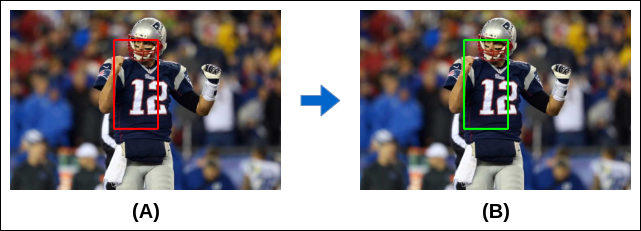
\includegraphics{6-Desenvolvimento-Projeto/imagens-desenvolvimento/representacao_numero.png}}
	\end{center}
	\centering \legend{Fonte: Elaborada pelos autores.}
\end{figure}

A \autoref{ambiente_de_testes} mostra quais ambientes foram escolhidos para realizas os testes do \textit{software}:

\begin{table}[h]
\centering
\caption{Ambiente de testes}
\label{ambiente_de_testes}
\begin{tabular}{l|l|l} 
\hline
\hline
\multicolumn{1}{l|}{Ambiente} & Iluminação & \multicolumn{1}{l}{Possível resultado}  \\ 
\hline
Partida de futebol americano   & Boa        & Positivo                                 \\
Partida de futebol americano   & Baixa      & Negativo                                 \\
Jogador parado                 & Boa        & Positivo                                 \\
Jogador em movimento (Lento)   & Boa        & Intermediário                            \\
Jogador de frente              & Boa        & Positivo                                 \\
Jogador de costas              & Boa        & Positivo \\
\hline
\hline 
\end{tabular}
\end{table}